\documentclass[runningheads]{llncs}

\usepackage{graphicx}
\usepackage{listings}
% Used for displaying a sample figure. If possible, figure files should
% be included in EPS format.
%
% If you use the hyperref package, please uncomment the following line
% to display URLs in blue roman font according to Springer's eBook style:
% \renewcommand\UrlFont{\color{blue}\rmfamily}

% Copyright 2017 Sergei Tikhomirov, MIT License
% https://github.com/s-tikhomirov/solidity-latex-highlighting/

\usepackage{listings, xcolor}

\definecolor{verylightgray}{rgb}{.97,.97,.97}

\lstdefinelanguage{Solidity}{
	keywords=[1]{anonymous, assembly, assert, balance, break, call, callcode, case, catch, class, constant, continue, contract, debugger, default, delegatecall, delete, do, else, emit, event, export, external, false, finally, for, function, gas, if, implements, import, in, indexed, instanceof, interface, internal, is, length, library, log0, log1, log2, log3, log4, memory, modifier, new, payable, pragma, private, protected, public, pure, push, require, return, returns, revert, selfdestruct, send, storage, struct, suicide, super, switch, then, this, throw, transfer, true, try, typeof, using, value, view, while, with, addmod, ecrecover, keccak256, mulmod, ripemd160, sha256, sha3}, % generic keywords including crypto operations
	keywordstyle=[1]\color{blue}\bfseries,
	keywords=[2]{address, bool, byte, bytes, bytes1, bytes2, bytes3, bytes4, bytes5, bytes6, bytes7, bytes8, bytes9, bytes10, bytes11, bytes12, bytes13, bytes14, bytes15, bytes16, bytes17, bytes18, bytes19, bytes20, bytes21, bytes22, bytes23, bytes24, bytes25, bytes26, bytes27, bytes28, bytes29, bytes30, bytes31, bytes32, enum, int, int8, int16, int24, int32, int40, int48, int56, int64, int72, int80, int88, int96, int104, int112, int120, int128, int136, int144, int152, int160, int168, int176, int184, int192, int200, int208, int216, int224, int232, int240, int248, int256, mapping, string, uint, uint8, uint16, uint24, uint32, uint40, uint48, uint56, uint64, uint72, uint80, uint88, uint96, uint104, uint112, uint120, uint128, uint136, uint144, uint152, uint160, uint168, uint176, uint184, uint192, uint200, uint208, uint216, uint224, uint232, uint240, uint248, uint256, var, void, ether, finney, szabo, wei, days, hours, minutes, seconds, weeks, years},	% types; money and time units
	keywordstyle=[2]\color{teal}\bfseries,
	keywords=[3]{block, blockhash, coinbase, difficulty, gaslimit, number, timestamp, msg, data, gas, sender, sig, value, now, tx, gasprice, origin},	% environment variables
	keywordstyle=[3]\color{violet}\bfseries,
	identifierstyle=\color{black},
	sensitive=false,
	comment=[l]{//},
	morecomment=[s]{/*}{*/},
	commentstyle=\color{gray}\ttfamily,
	stringstyle=\color{red}\ttfamily,
	morestring=[b]',
	morestring=[b]"
}

\lstset{
	language=Solidity,
	backgroundcolor=\color{verylightgray},
	extendedchars=true,
	basicstyle=\footnotesize\ttfamily,
	showstringspaces=false,
	showspaces=false,
	numbers=left,
	numberstyle=\footnotesize,
	numbersep=9pt,
	tabsize=2,
	breaklines=true,
	showtabs=false,
	captionpos=b
}


\begin{document}
%
\title{Untrusted B2B Collaboration using the Blockchain}
%
%
\author{Jonas Beyer \and Philipp Otto \and S\"oren Tietb\"ohl}
%
\authorrunning{J. Beyer et al.}
%
\institute{
	Hasso-Plattner-Institut, Potsdam, Germany\\
	\email{\{jonas.beyer,philipp.otto2,soeren.tietboehl\}@student.hpi.de}}
%
\maketitle % typeset the header of the contribution
%
\begin{abstract}
	Lack of trust between communication partners is one of the major issues companies face when implementing business processes in a cross-organizational setting.
	Blockchain is an emerging technology that enables decentralization and distribution of state without the need for a trusted central instance.
	As a result, it is possible to form consensus in the communication between otherwise untrusting parties.
	In this paper we introduce Armadillo, an open-source prototype implementation for realizing business process choreographies using the Ethereum blockchain.
	We present a user interface for connecting business processes with blockchain calls, as well as an underlying smart contract structure for inter-process communication.

	\keywords{Business Processes \and BPMN \and Choreographies \and Blockchain \and Ethereum \and Smart Contracts}
\end{abstract}
%
%
%
\section{Introduction}

% Establish common ground with reader Worth readers time? Give some results

% Write it once at the start, then rewrite at the end
% use it to guide paper

% Important -> this structure will be expected

% Context (Topic / Terminology)
% Problem & Relevance (Problem - Costs / Current state - Gain)
% Related Work (Existing solutions / Shortcomings)
% Goals / Claims (Contribution, Sketch Results)
% Paper structure (The remainder of this paper is structured as follows ...)

% What is BPMN?
The Business Process Model Notation (BPMN) enables detailed documentation of business processes. This is used to realize complex inter-business processes which involve vast communication structures. One common problem is that within these processes the parties have to trust each other.
% What is Blockchain?

With the increasing spread of Blockchain technology, this problem could be rectified.
A Blockchain is a decentralized information-storage network. Information is stored in blocks, which are chained together via cryptograhic means. This means, that many participants can agree on a common public state of information without trusting each other. This technology is commonly used to realize virtual currencies, also called cryptocurrencies.
Ethereum is one implementation of the Blockchain concept, and it realizes a key feature called smart contracts.
Smart contracts are small programs, which are ran by the Blockchain network. They have very limited processing power, but they enable the execution of code which has a commonly known state.

%What problems are there with BPMN that can be solved with Blockchain?
The problem of needing to trust each other when collaborating in a business process can be addressed by applying the benefits of blockchain technology. The Blockchain be used in several ways to facilitate trusted communication between untrusted parties.

% What approaches exist currently (Caterpillar \cite{lopez2017caterpillar}, Untrusted paper \cite{weber2016untrusted})
Current approaches aim to convert the functionality of traditional BPMN Engines to smart contracts on the Ethereum Blockchain.

Caterpillar~\cite{lopez2017caterpillar} features the implementation of most common BPMN elements. It enables the transformation of BPMN Models to smart contracts, which can be deployed and executed on the Blockchain.

Weber et al.~\cite{weber2016untrusted} realize Orchestrations on the Blockchain.

%What is our general Idea?
We want to expand on the work of Weber et al. and implement true choreographies. In their current approach they are using one central smart contract called a mediator / monitor which manages the Orchestration state.
We will have a set of smart contracts for every party, which will then communicate with each other to realize the choreography.
%What are our results? (briefly)

\section{Preliminary}
In the following section we present concepts and technologies that are related to our concept.

\subsection{Orchestrations and Choreographies}

\subsection{Blockchain}
A blockchain is a distributed ledger that allows users to find a concensus in decentralized applications.
It works by splitting information into blocks that are connected as a linked list.
%TODO proof of work is only one possibility
%TODO explain more in depth?
Each block has to be signed in a way that is mathematically hard to calculate, but easy to verify.
Therefore users can verify if their local blockchain is valid.
If the same block is signed at the same time, a fork of the blockchain can happen, i.e. two versions of the same blockchain exist at the same time.
A concensus is reached by propagating the longest blockchain within the network until it is accepted by all parties of the network.

%TODO reference original blockchain paper
Blockchain technology is used in cryptocurrencies, most notably Bitcoin \cite{nakamoto2008bitcoin}.
The use in cryptocurrency has laid the foundation for a number of decentralized application besides financial ones.
Ethereum \cite{wood2014ethereum} is a cryptocurrency that also builds on blockchain technologies and allows users to execute code in the form of \emph{smart contracts}.
Smart contracts are Turing complete code artifacts, that can be deployed on the blockchain and have an interface that is callable by users.
They can receive and send money, store information locally and emit events on the blockchain ledger.
When calling functions on a smart contract, users have to supply \emph{gas}, a unit that powers smart contract computations.
Contracts deplete gas for each operation and return excess gas back to the user.
This ensures that contracts are not running for an unlimited amount of time and that computations on the blockchain are expensive in order to avoid unnecessary operations being performed on-chain.
%TODO short text on the paper which shows smart contract examples
%TODO short text on solidity

\subsection{Prior Work on Business Processes on the Blockchain}
In \cite{weber2016untrusted}, a first approach of monitoring and coordinating business process interactions across organizations on the blockchain was presented.
Using a smart contract as a central \emph{monitor} or \emph{mediator} of the communication, a form of inter-process orchestration is implemented.
They describe a contract architecture, where a factory contract is responsible for deploying instance contracts for each process instance.
They also introduce the concept of \emph{triggers}, applications that listen to events on the blockchain and trigger external API calls.
In order to achieve BPMN-to-Solidity compilation, they describe translation rules to transform BPMN elements to Solidity code.
%TODO highlight lack of access right explanation and problem of central contract?

%we build on:
%factories \& instances
%registering users to roles
%triggers
%the model they used (originally from Fdhila et al)

%we don\'t:
%do bpmn solidity translation
%use one central contract instance

%summarize Caterpillar
%acknowledge their Work
%display the shortcomings
\cite{lopez2017caterpillar} presents an open-source implementation of an Ethereum-based Business Process Management System.
It implements BPMN-to-Solidity compilation and thereby tracks the state of process executions on the blockchain.
Processes can be started and executed via a user interface, which calls the generated Solidity code in the background.

%describes components and architecture of engine
%automatic bpmn solidity translation
%no choreographies / lanes supported, all tasks / transitions are managed on-chain through process %contract

\section{Solution approach}
We propose a system design, that allows choreographies to be executed publicly on the blockchain.
In the following section, we describe our approach and its architecture.

%basic understanding/ intuition
%-> make orchestration possible

% Decentralized contracts vs. central monitor
% Engine on chain vs. message channel

%use one contuous example

%visualizations !!

\subsection{System overview}
\begin{figure}
	\centering
	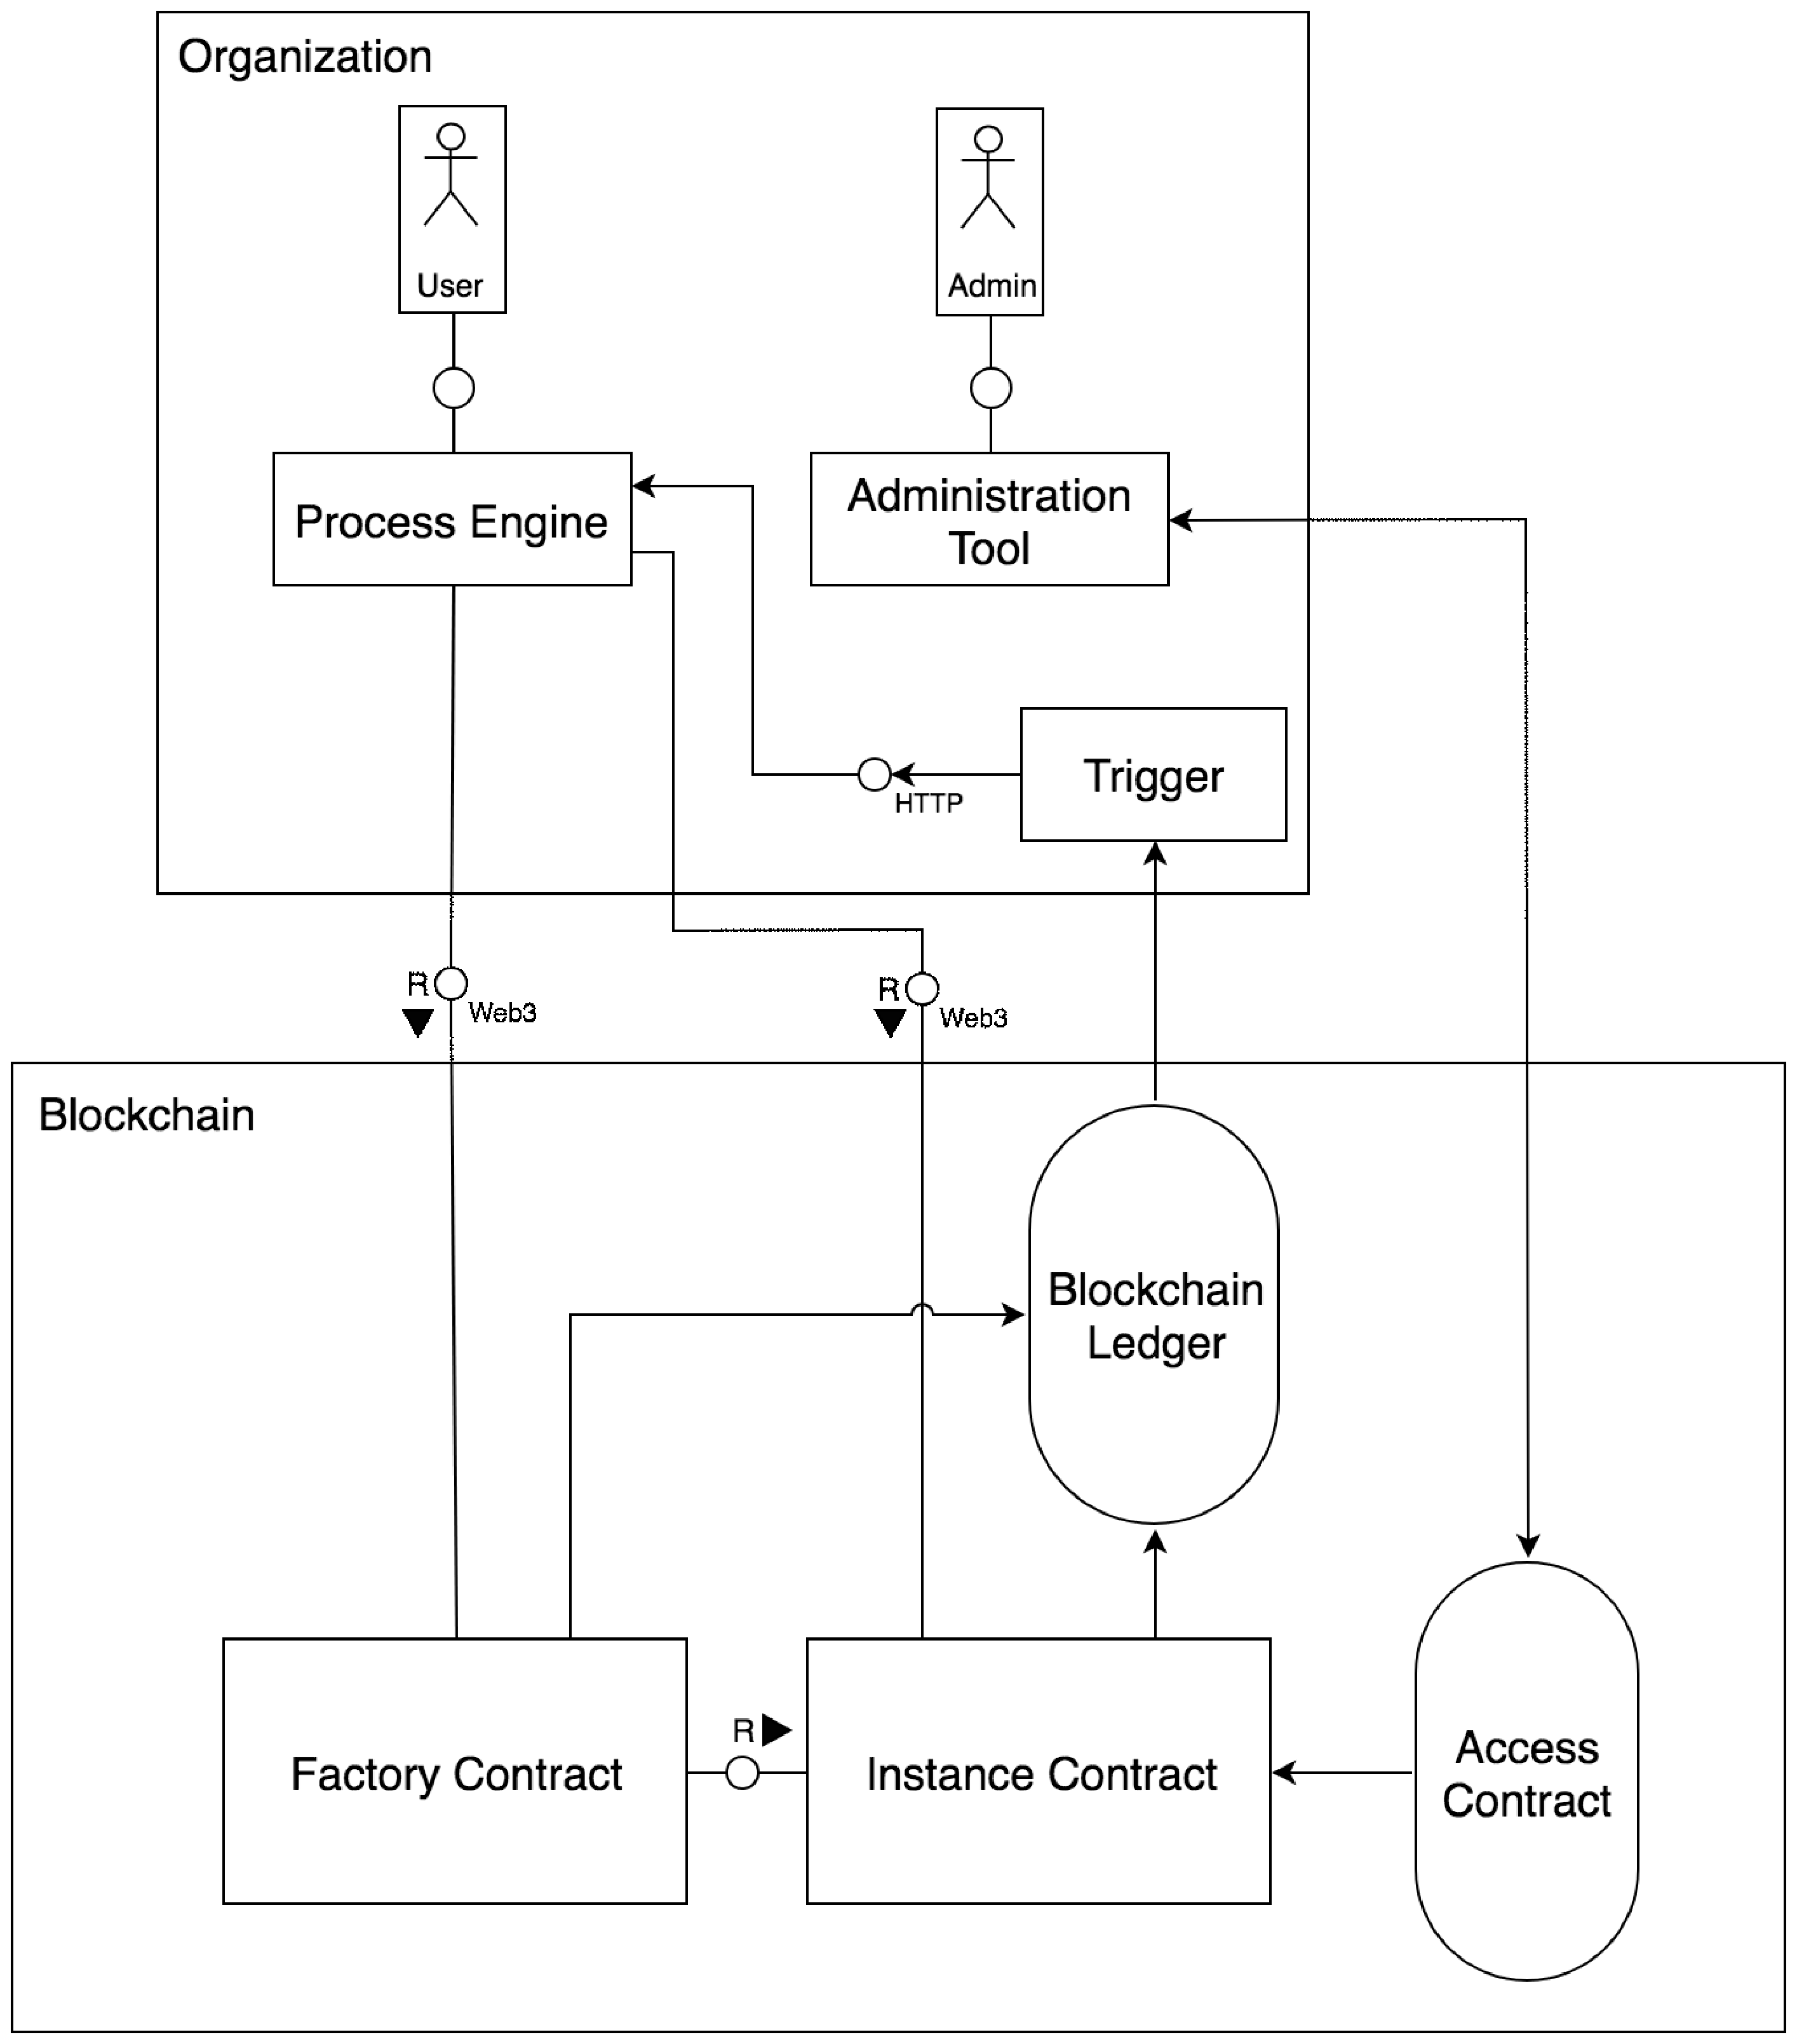
\includegraphics[width=100mm]{fig/system_diagram.eps}
	\caption{An architecture diagram showing the interactions within the system.} 			
	\label{fig:system_diagram}
\end{figure}

Every organization provides an interface of their public process in an \emph{instance contract}.
Additionally, \emph{factory contracts} manage these instance contracts and \emph{access contracts} are used for rights management.
The contract structure will be described in detail in the following sections.
We assume that all participating organizations use a process engine to execute their private processes.
When a throw event is triggered within a process engine, a \emph{throw event function} is called on an instance contract and the corresponding \emph{catch event function} is called on the instance contract of the organization responsible for catching the event.
Thus, the public processes of all organizations are recorded on the blockchain.

%TODO reference "trigger" from Untrusted paper
Each organization uses a \emph{trigger} that continuously listens to catch events.
If a catch event is observed, this information is relayed to the process engine to handle the event.
The usage of the blockchain to monitor the choreography is encapsulated in the process engine and is therefore hidden from the users.

The interaction of the components can be seen in Figure \ref{fig:system_diagram}.

\subsection{Contract Structure}
To realize the system, we use three kinds of smart contracts.
Firstly, each organization uses one \emph{instance contract} per process instance.
It represents the public process of the organization for the corresponding process.
It is called during the process execution when a catch or throw event is reached in the process instance.
When this happens, it emits an event on the blockchain to document this fact.

Secondly, each organization uses one \emph{factory contract} per process.
It is responsible for creating instance contracts and saving a mapping from instance IDs to the corresponding contracts.

Thirdly, each organization uses \emph{access contracts} to manage which users can trigger events on the instance contracts.
Either, there is on access contract per process or access contracts are shared over multiple processes depending on the use case.

\subsection{Per company setup}
\begin{figure}
	\centering
	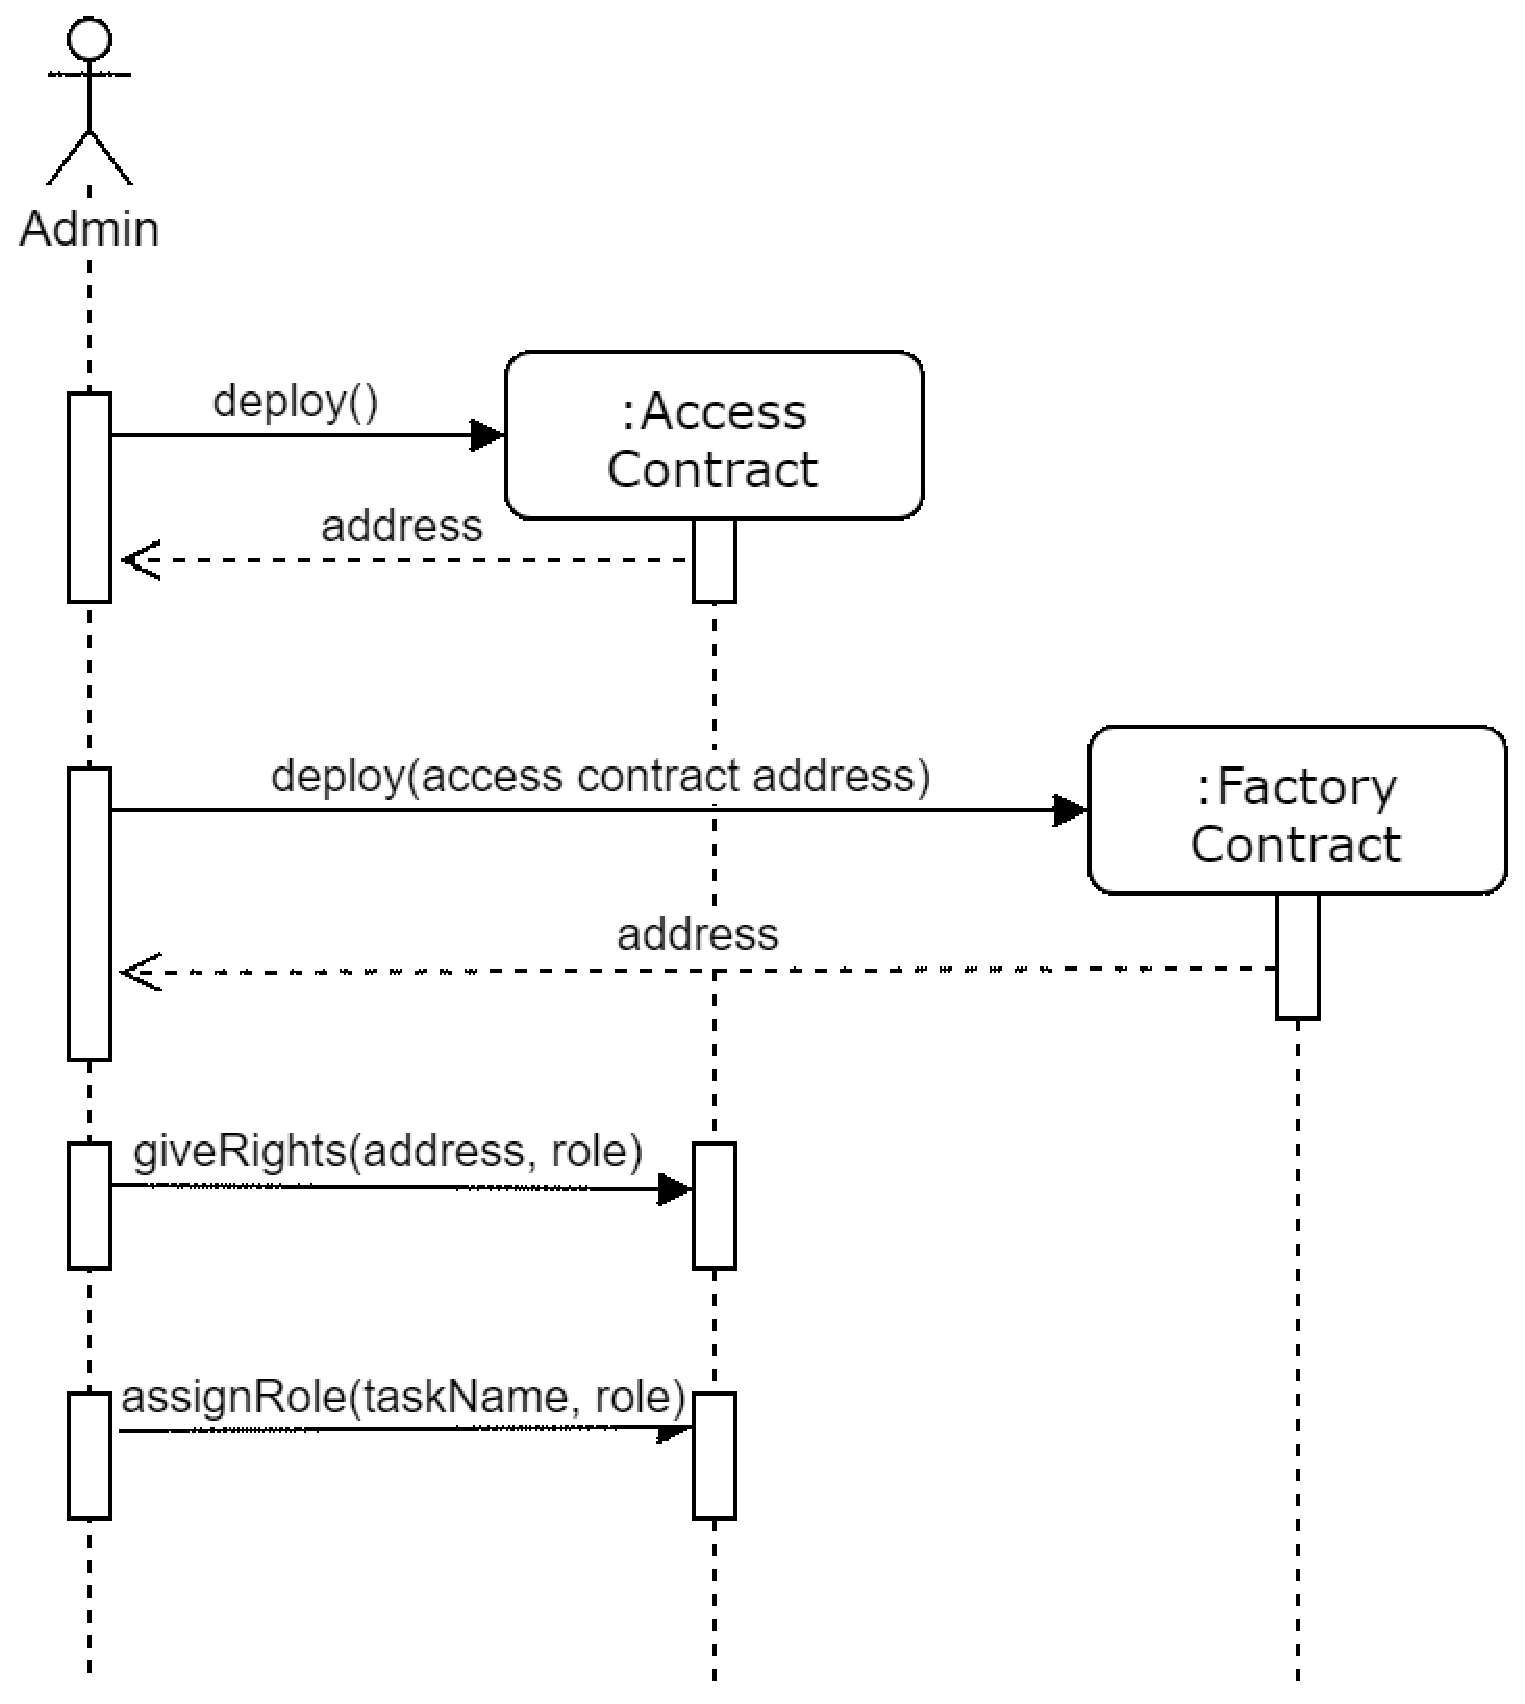
\includegraphics[width=70mm]{fig/initialization.eps}
	\caption{A sequence diagram describing the initialization process for an organization.} 
	\label{fig:initialization}
\end{figure}

%TODO add a step where other factory contracts are set
Each organization needs to perform some setup before they can take part in a process execution.
An access contract and a factory contract for a process need to be deployed it it has not been done yet.
Additionally, the user-to-role and and task-to-role mappings have to be updated, to allow verification of users during the process execution.
A diagram of this process can be seen in Figure \ref{fig:initialization}.

\subsection{Interaction setup}
\begin{figure}
	\centering
	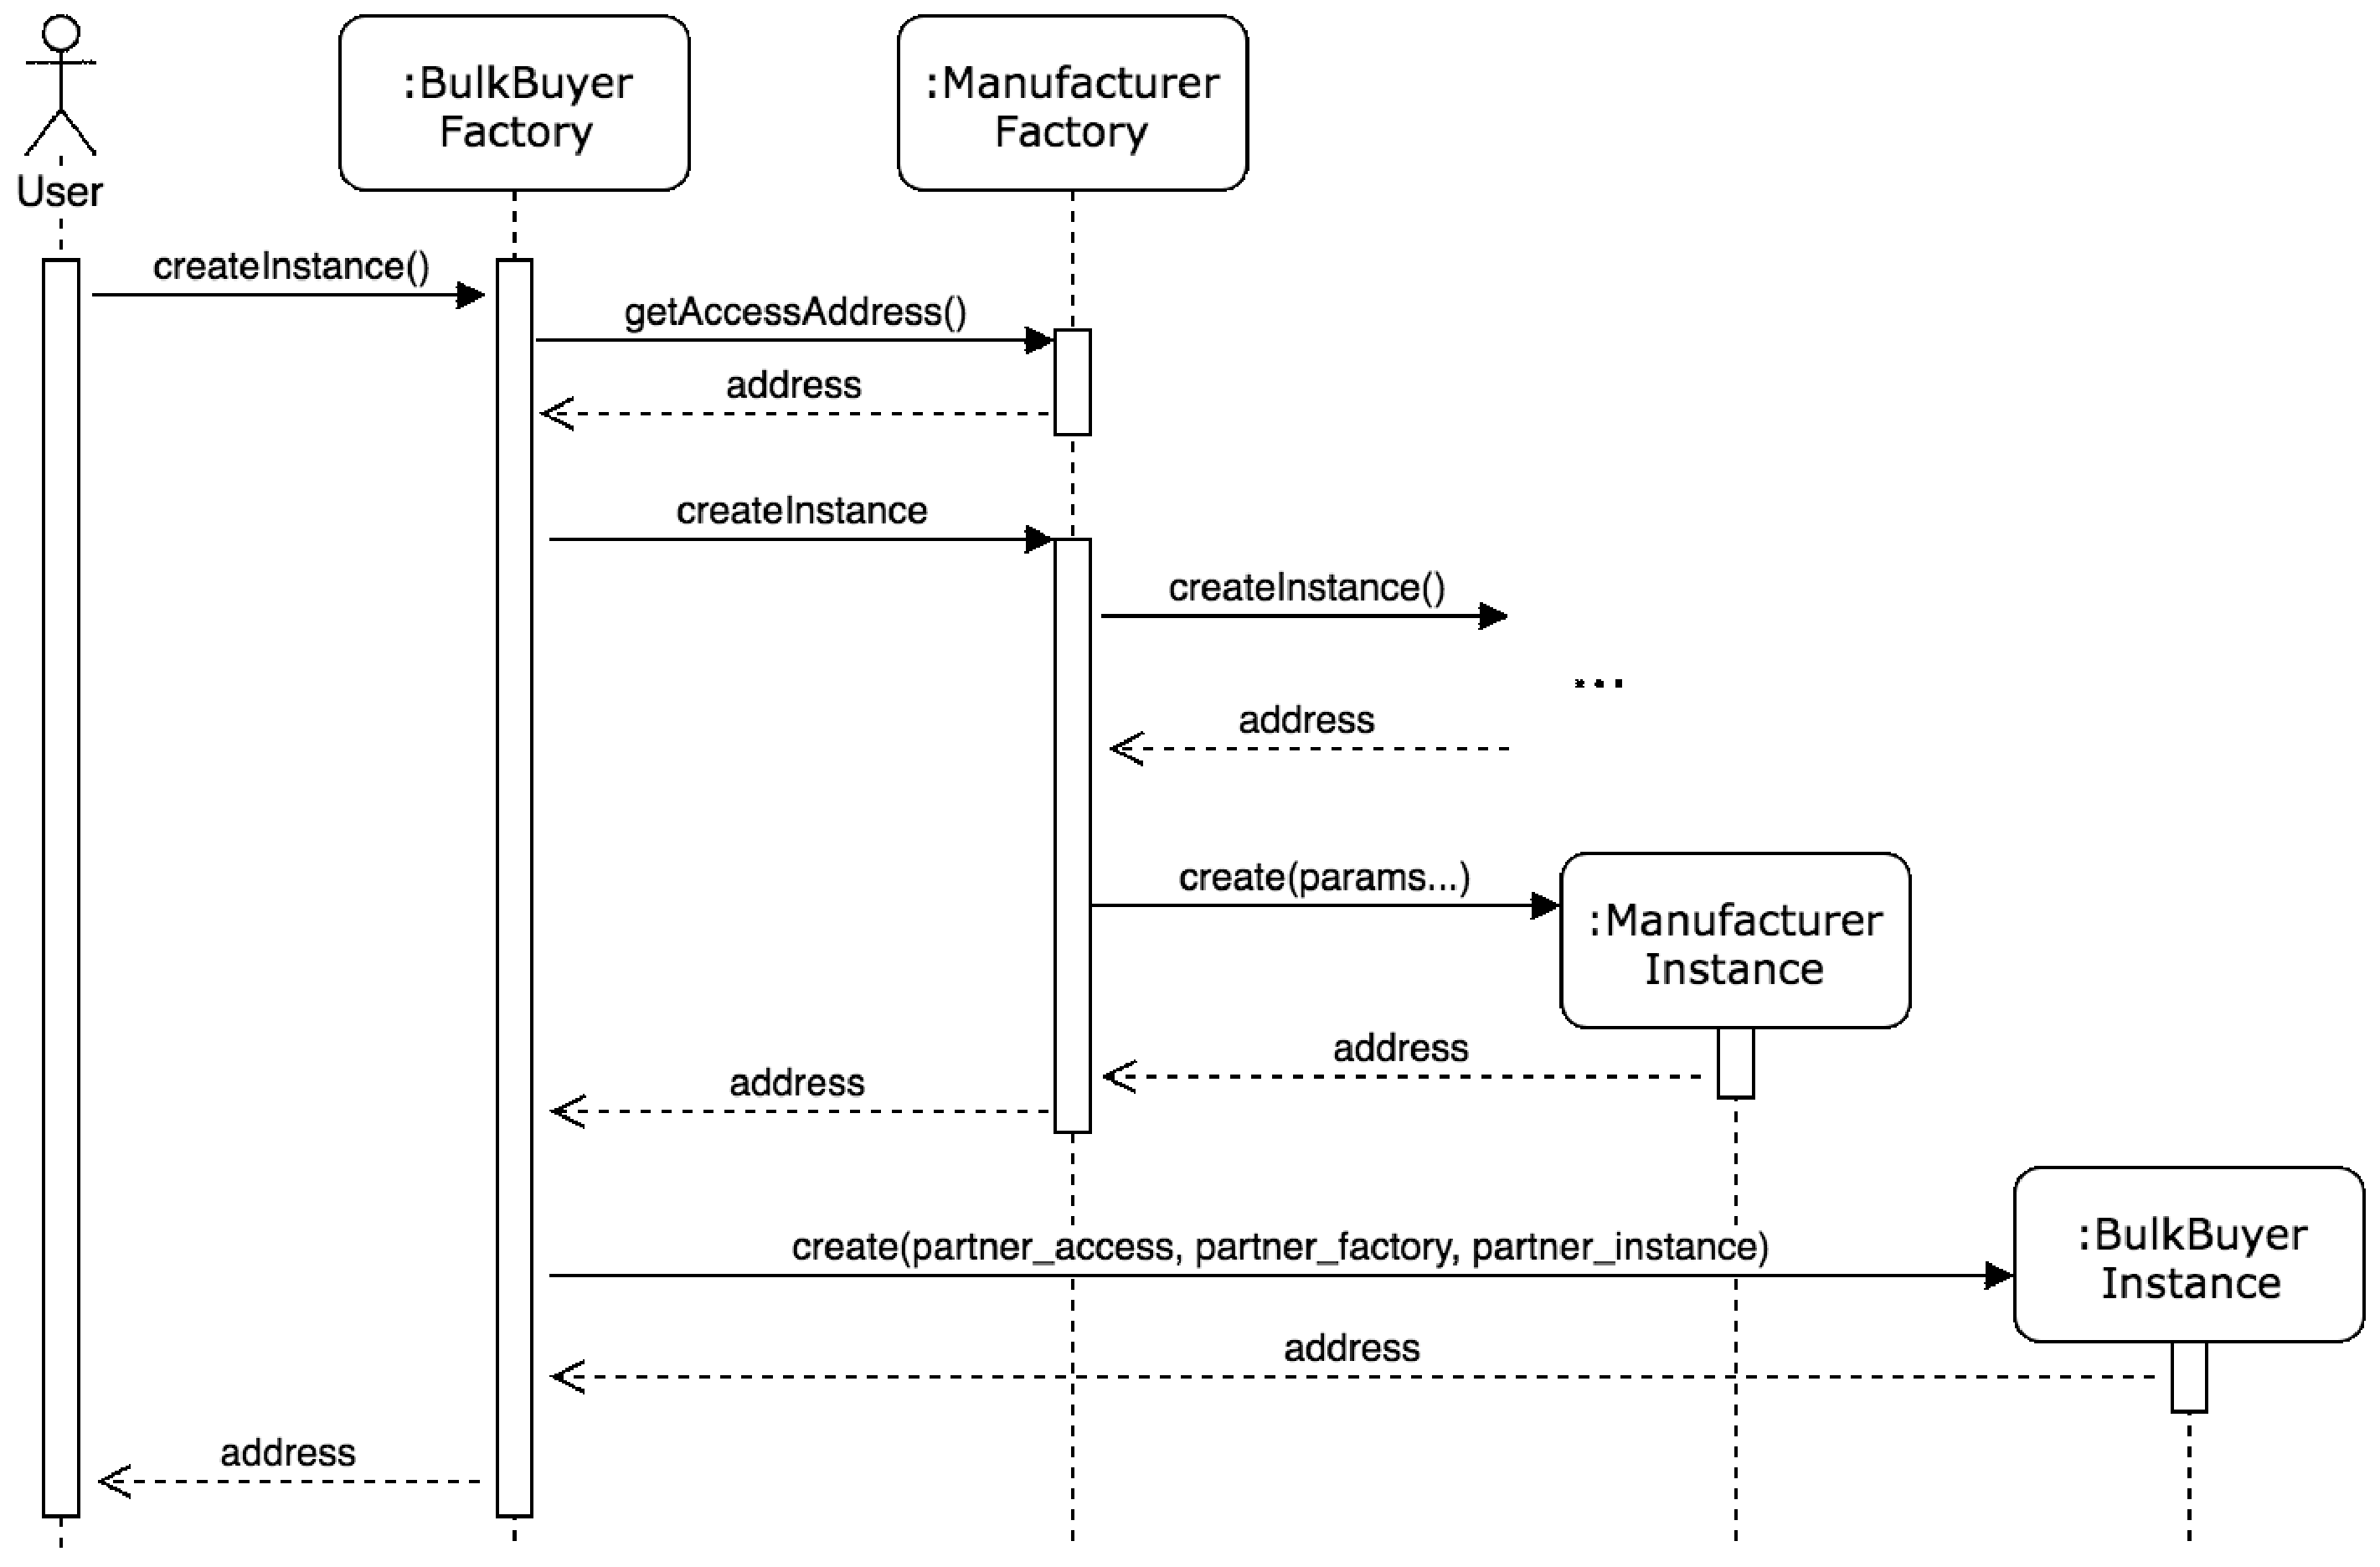
\includegraphics[width=\textwidth]{fig/instance_creation.eps}
	\caption{A sequence diagram describing the process of creating a new process instance.} 
	\label{fig:instance_creation}
\end{figure}

In order to create a new process instance, the organization that initiates the instance by triggering the first throw event has to explicitly create an instance contract by calling the factory contract.
To create an instance contract, the factory contract may need to initialize other instance contracts by calling other factory contracts.
When all partner instance, factory and access contracts are known, the instance contract can be created and its address is returned to the user and an event is emitted to the blockchain.
This process is visualized in Figure \ref{fig:instance_creation}.

The recursive initialization ensures that all instance contracts that are part of the process instance will be created by one function call.
%TODO add emit event in the diagram
%TODO better formulation
The organizations that did not start the instance creation can detect the new process instance by using their trigger to watch the factory contract.

\subsection{Sending messages}
\begin{figure}
	\centering
	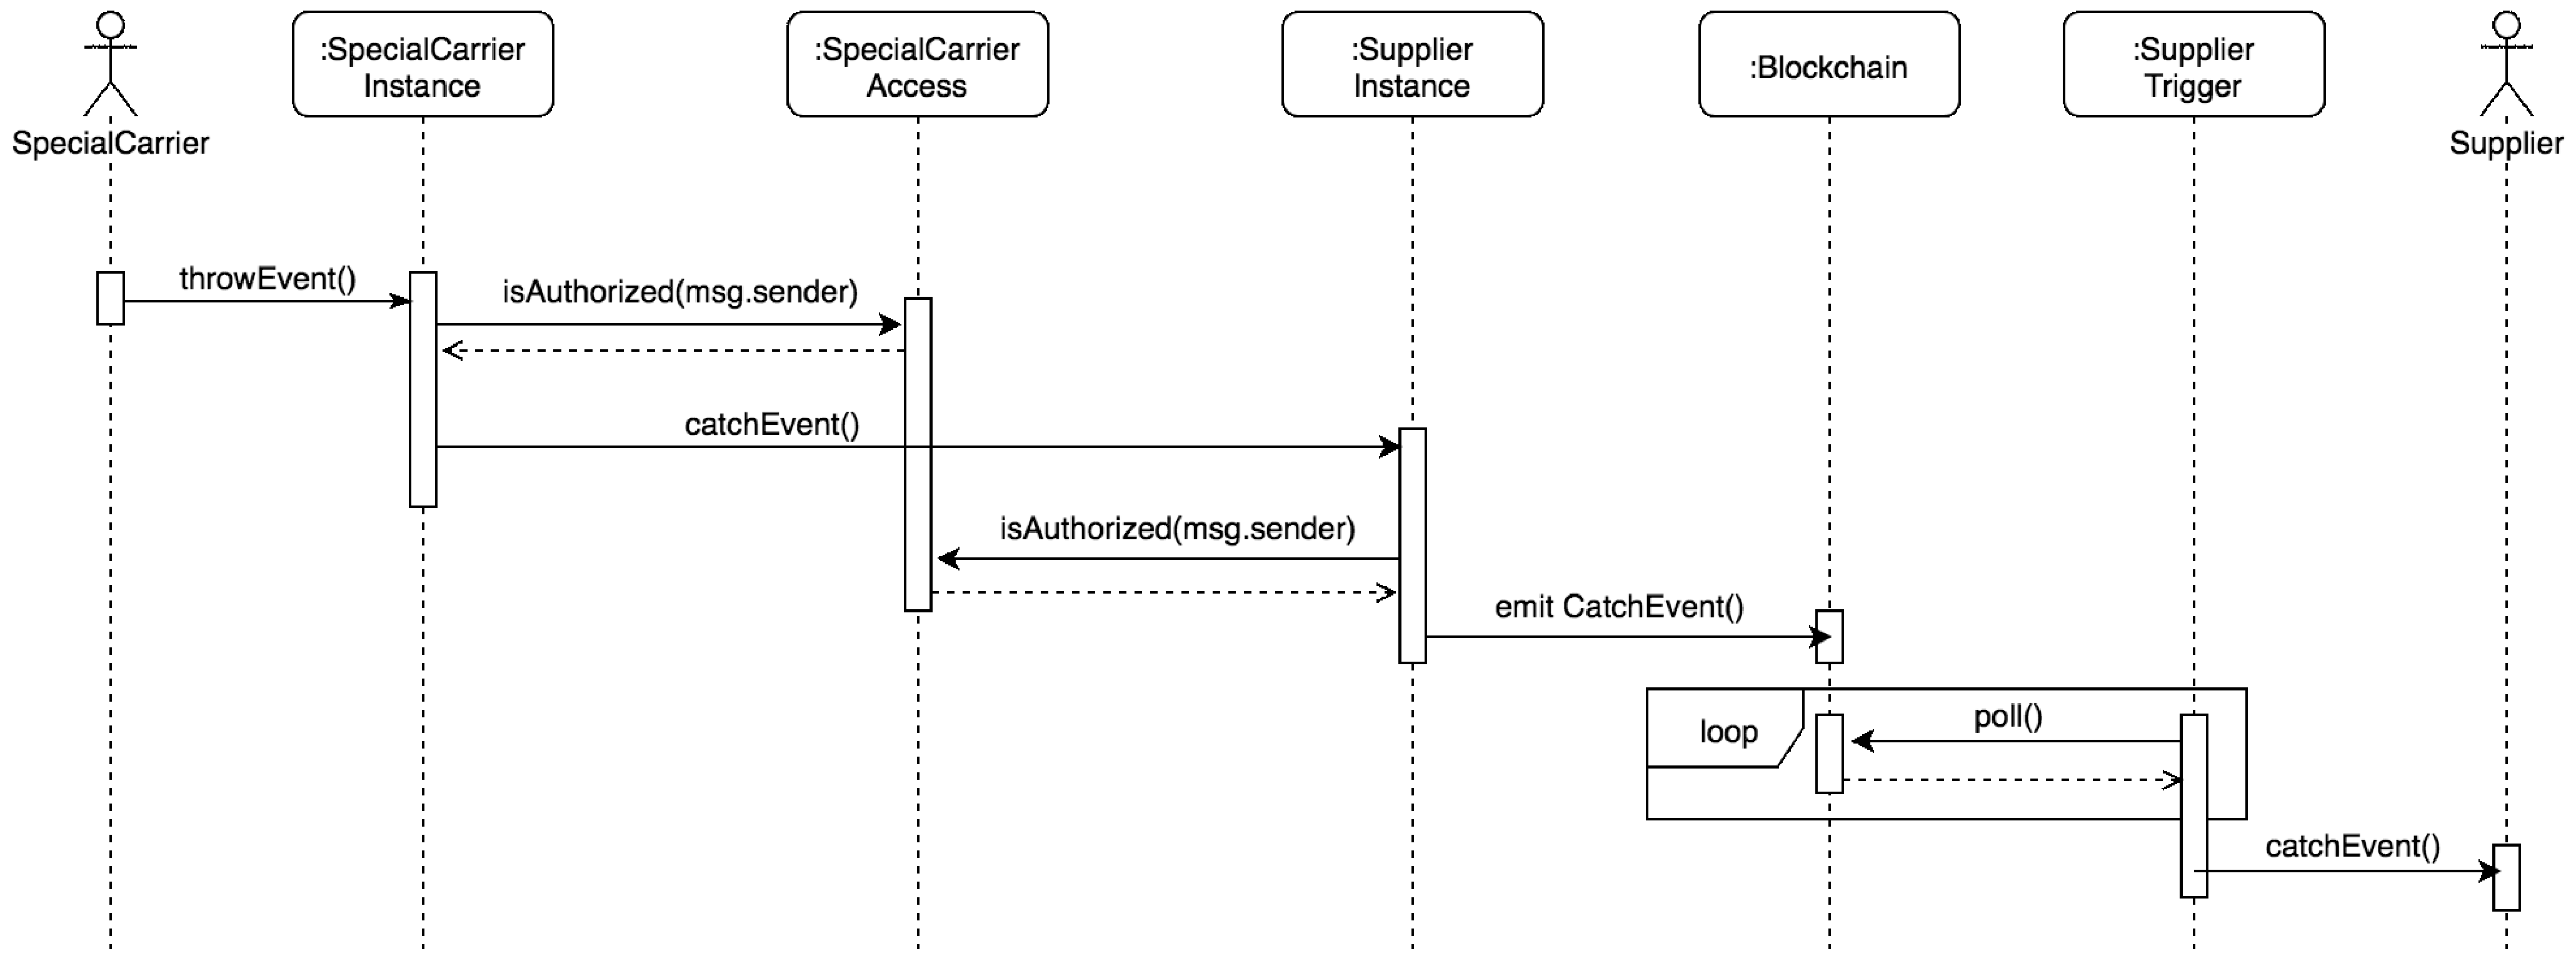
\includegraphics[width=\textwidth]{fig/event_sending.eps}
	\caption{A sequence diagram describing the process of sending a message to a collaboration partner.} 
	\label{fig:event_sending}
\end{figure}

%TODO correctly show that the address is passed instead of using msg.sender
When a throw event is triggered in the process engine of organization $A$, the corresponding \emph{throw event function} is called on the instance contract of the collaboration partner $B$.
In the instance contract of $A$ an authorization is performed by looking up the sender address in the access contract of $A$.
If this check is successful, the \emph{catch event function} is called on the partner instance contract of $B$.
In the instance contract of $B$ there is another authorization against the access contract of $A$.
This ensures that both sides can be confident, that the throw event was triggered by an authorized person who belongs to organization $A$.
If this check was also successful, an event is emitted to the blockchain.
This will be detected by the trigger of $B$ and passed to the process engine.
Thus, a message was sent from $A$ to $B$ via the blockchain and an audit trail was created.
An example can be seen in the sequence diagram in Figure \ref{fig:event_sending}.


\section{Implementation}

Given the architecture, we will now discuss the implementation of the contracts used in the system.
Afterwards, we will shortly describe the tools we built for interacting with the system.

\subsection{Contracts}

\subsubsection{Process Contracts}

For taking part in the process collaboration, each company needs to deploy a factory contract that contains the contract definition of the company's instance contract.
This closely follows the factory contract pattern used in \cite{weber2016untrusted}, and described as Pattern 14 in \cite{xu2018pattern}.

- Split between choreography intiator and other participants
- has following interface:
- constructor, passing the address of the access contract (needs to deployed first, details in next section)
- setters for dependent factories
- createInstance()
- getAccessAddress()
- isInstance(id, address)
- has following internal impl
- guard instance creation until all dependent factories are set
-> hold list of addresses of dependent factories
- hold address of access contract
- hold mapping from uuid -> address, identifying its own instances for a given choreography id
- if initiator: generate uuid on createInstance

The factory contract source code also contains the public interfaces of
- the access contract (same for every participant)
- remote factory contracts (if receiving messages from remote, for verification)
- remote instance contracts (if sending messages to remote instance)
as well as the complete definition of the instance contract source code.

The instance contract provides the following interface
- a constructor where the local access contract, the choreography id and all dependency addresses can be passed
- a function for each sending action (task or event), called from process engine
- a function for each receiving action (task or event), called from other instance contracts
and the following internal impl
- hold the choreography id
- hold the addresses of its own factory (for selfdestruction) and its own access contract (for local verification)
- hold the addresses of remote factory and access contract (again, if receiving messages from remote)
- hold the addresses of remote instance contract (again, if sending messages)
- add guards to each sending action to verify the local sender
- add guards to each receiving action to verify the remote sender
- implement events and emit them to the blockchain on receive action, that can be watched from external triggers
- call remote receive functions on local send action
- selfdestruct on the last send or receive action of the instance

Guards = access checks (Pattern 13)

See github repo for example % TODO

\subsubsection{Access Contract}

Each company deploys an access contract that holds information about the roles and permissions of the company's employees.
Having permission data encapsuled in a separate access contract follows pattern 12, the Data Contract pattern, from \cite{xu2018pattern}.
It allows decoupling the roles and permissions from the actual contract instances, allowing for a simple modification at runtime.
Access contracts can be deployed per process, or even once per company as a single source of truth for all processes.

To allow the administration of user permissions, access contracts provide the following interface:
\begin{itemize}
	\item
	      \texttt{assignRoleToUser(userAddress, role)}
	\item
	      \texttt{removeRoleFromUser(userAddress, role)}
	\item
	      \texttt{assignTaskToRole(task, role)}
	\item
	      \texttt{removeTaskFromRole(task, role)}
\end{itemize}
The access to these functions should be guarded, allowing only a specific administrator address to call them.

Verifying a users permission to execute a certain task can be achieved by calling \texttt{isAuthorized(userAddress, task)}.
\newline

Given this interface, there are multiple possible implementation approaches for access contracts.
As it was our main focus to develop a running prototype, and not to provide an optimized, production-ready system, we decided on a simple mapping-based implementation:
\begin{lstlisting}[
  caption=Mappings in our access contract implementation,
  language=Solidity,
  basicstyle=\small
]
pragma solidity ^0.4.23;

contract Access {
    mapping(string => string) taskToRole;
    mapping(string => uint) roleToIndex;
    mapping(address => uint) addressToAccessBitmask;
    ...
}
\end{lstlisting}
The first mapping stores the tasks that can be executed by a specific role (cf. pools and lanes, and their contained tasks, in BPMN diagrams).
The second mapping assigns each role an index in the access bitmask, i.e., if the bit at the given index is set, the user holds the corresponding role.
The third mapping assigns such an access bitmask to each user.

Storing large amounts data on the blockchain is expensive by design.
As the mappings grow in size with each user, role and task that is part of some process in the company, our implementation is probably not suited for real-world application.
Finding optimized, less costly (both in computation cost and storage cost) approaches is part of future work.
One other approach we thought of is based on Pattern 5 of \cite{xu2018pattern} - depicting real world permissions as tokens, and "paying" with these tokens on function call to verify one's role.

\subsection{Tools}

\subsubsection{eth\_admin}

node-js command line tool using vorpal
commands trigger blockchain calls using web3

\subsubsection{armadillo}

\section{Evaluation}
%Gas cost
%Time for one instance
%Setup difficulty
%Security

%Mention problem of giving and removing right to change access rights
%But in the end one instance has to a be superadmin in the contract, if it is leaked there is a problem

% future work: 
% - access contract
% - instantiation
% - automatic generation -> template
\section{Conclusion}

%
% ---- Bibliography ----
%
% BibTeX users should specify bibliography style 'splncs04'.
% References will then be sorted and formatted in the correct style.
%
\bibliographystyle{splncs04}
\bibliography{references}

\end{document}
